\documentclass[conference]{IEEEtran}
% Some Computer Society conferences also require the compsoc mode option,
% but others use the standard conference format.
%
% If IEEEtran.cls has not been installed into the LaTeX system files,
% manually specify the path to it like:
% \documentclass[conference]{../sty/IEEEtran}





% Some very useful LaTeX packages include:
% (uncomment the ones you want to load)


% *** MISC UTILITY PACKAGES ***
%
%\usepackage{ifpdf}
% Heiko Oberdiek's ifpdf.sty is very useful if you need conditional
% compilation based on whether the output is pdf or dvi.
% usage:
% \ifpdf
%   % pdf code
% \else
%   % dvi code
% \fi
% The latest version of ifpdf.sty can be obtained from:
% http://www.ctan.org/pkg/ifpdf
% Also, note that IEEEtran.cls V1.7 and later provides a builtin
% \ifCLASSINFOpdf conditional that works the same way.
% When switching from latex to pdflatex and vice-versa, the compiler may
% have to be run twice to clear warning/error messages.






% *** CITATION PACKAGES ***
%
%\usepackage{cite}
% cite.sty was written by Donald Arseneau
% V1.6 and later of IEEEtran pre-defines the format of the cite.sty package
% \cite{} output to follow that of the IEEE. Loading the cite package will
% result in citation numbers being automatically sorted and properly
% "compressed/ranged". e.g., [1], [9], [2], [7], [5], [6] without using
% cite.sty will become [1], [2], [5]--[7], [9] using cite.sty. cite.sty's
% \cite will automatically add leading space, if needed. Use cite.sty's
% noadjust option (cite.sty V3.8 and later) if you want to turn this off
% such as if a citation ever needs to be enclosed in parenthesis.
% cite.sty is already installed on most LaTeX systems. Be sure and use
% version 5.0 (2009-03-20) and later if using hyperref.sty.
% The latest version can be obtained at:
% http://www.ctan.org/pkg/cite
% The documentation is contained in the cite.sty file itself.






% *** GRAPHICS RELATED PACKAGES ***
%
\ifCLASSINFOpdf
   \usepackage[pdftex]{graphicx}
  % declare the path(s) where your graphic files are
  % \graphicspath{{../pdf/}{../jpeg/}}
  % and their extensions so you won't have to specify these with
  % every instance of \includegraphics
  % \DeclareGraphicsExtensions{.pdf,.jpeg,.png}
\else
  % or other class option (dvipsone, dvipdf, if not using dvips). graphicx
  % will default to the driver specified in the system graphics.cfg if no
  % driver is specified.
   \usepackage[dvips]{graphicx}
  % declare the path(s) where your graphic files are
  % \graphicspath{{../eps/}}
  % and their extensions so you won't have to specify these with
  % every instance of \includegraphics
  % \DeclareGraphicsExtensions{.eps}
\fi
% graphicx was written by David Carlisle and Sebastian Rahtz. It is
% required if you want graphics, photos, etc. graphicx.sty is already
% installed on most LaTeX systems. The latest version and documentation
% can be obtained at: 
% http://www.ctan.org/pkg/graphicx
% Another good source of documentation is "Using Imported Graphics in
% LaTeX2e" by Keith Reckdahl which can be found at:
% http://www.ctan.org/pkg/epslatex
%
% latex, and pdflatex in dvi mode, support graphics in encapsulated
% postscript (.eps) format. pdflatex in pdf mode supports graphics
% in .pdf, .jpeg, .png and .mps (metapost) formats. Users should ensure
% that all non-photo figures use a vector format (.eps, .pdf, .mps) and
% not a bitmapped formats (.jpeg, .png). The IEEE frowns on bitmapped formats
% which can result in "jaggedy"/blurry rendering of lines and letters as
% well as large increases in file sizes.
%
% You can find documentation about the pdfTeX application at:
% http://www.tug.org/applications/pdftex





% *** MATH PACKAGES ***
%
%\usepackage{amsmath}
% A popular package from the American Mathematical Society that provides
% many useful and powerful commands for dealing with mathematics.
%
% Note that the amsmath package sets \interdisplaylinepenalty to 10000
% thus preventing page breaks from occurring within multiline equations. Use:
%\interdisplaylinepenalty=2500
% after loading amsmath to restore such page breaks as IEEEtran.cls normally
% does. amsmath.sty is already installed on most LaTeX systems. The latest
% version and documentation can be obtained at:
% http://www.ctan.org/pkg/amsmath





% *** SPECIALIZED LIST PACKAGES ***
%
%\usepackage{algorithmic}
% algorithmic.sty was written by Peter Williams and Rogerio Brito.
% This package provides an algorithmic environment fo describing algorithms.
% You can use the algorithmic environment in-text or within a figure
% environment to provide for a floating algorithm. Do NOT use the algorithm
% floating environment provided by algorithm.sty (by the same authors) or
% algorithm2e.sty (by Christophe Fiorio) as the IEEE does not use dedicated
% algorithm float types and packages that provide these will not provide
% correct IEEE style captions. The latest version and documentation of
% algorithmic.sty can be obtained at:
% http://www.ctan.org/pkg/algorithms
% Also of interest may be the (relatively newer and more customizable)
% algorithmicx.sty package by Szasz Janos:
% http://www.ctan.org/pkg/algorithmicx




% *** ALIGNMENT PACKAGES ***
\usepackage{booktabs}
\usepackage{array}
% Frank Mittelbach's and David Carlisle's array.sty patches and improves
% the standard LaTeX2e array and tabular environments to provide better
% appearance and additional user controls. As the default LaTeX2e table
% generation code is lacking to the point of almost being broken with
% respect to the quality of the end results, all users are strongly
% advised to use an enhanced (at the very least that provided by array.sty)
% set of table tools. array.sty is already installed on most systems. The
% latest version and documentation can be obtained at:
% http://www.ctan.org/pkg/array


% IEEEtran contains the IEEEeqnarray family of commands that can be used to
% generate multiline equations as well as matrices, tables, etc., of high
% quality.




% *** SUBFIGURE PACKAGES ***
%\ifCLASSOPTIONcompsoc
%  \usepackage[caption=false,font=normalsize,labelfont=sf,textfont=sf]{subfig}
%\else
%  \usepackage[caption=false,font=footnotesize]{subfig}
%\fi
% subfig.sty, written by Steven Douglas Cochran, is the modern replacement
% for subfigure.sty, the latter of which is no longer maintained and is
% incompatible with some LaTeX packages including fixltx2e. However,
% subfig.sty requires and automatically loads Axel Sommerfeldt's caption.sty
% which will override IEEEtran.cls' handling of captions and this will result
% in non-IEEE style figure/table captions. To prevent this problem, be sure
% and invoke subfig.sty's "caption=false" package option (available since
% subfig.sty version 1.3, 2005/06/28) as this is will preserve IEEEtran.cls
% handling of captions.
% Note that the Computer Society format requires a larger sans serif font
% than the serif footnote size font used in traditional IEEE formatting
% and thus the need to invoke different subfig.sty package options depending
% on whether compsoc mode has been enabled.
%
% The latest version and documentation of subfig.sty can be obtained at:
% http://www.ctan.org/pkg/subfig




% *** FLOAT PACKAGES ***
%
%\usepackage{fixltx2e}
% fixltx2e, the successor to the earlier fix2col.sty, was written by
% Frank Mittelbach and David Carlisle. This package corrects a few problems
% in the LaTeX2e kernel, the most notable of which is that in current
% LaTeX2e releases, the ordering of single and double column floats is not
% guaranteed to be preserved. Thus, an unpatched LaTeX2e can allow a
% single column figure to be placed prior to an earlier double column
% figure.
% Be aware that LaTeX2e kernels dated 2015 and later have fixltx2e.sty's
% corrections already built into the system in which case a warning will
% be issued if an attempt is made to load fixltx2e.sty as it is no longer
% needed.
% The latest version and documentation can be found at:
% http://www.ctan.org/pkg/fixltx2e


%\usepackage{stfloats}
% stfloats.sty was written by Sigitas Tolusis. This package gives LaTeX2e
% the ability to do double column floats at the bottom of the page as well
% as the top. (e.g., "\begin{figure*}[!b]" is not normally possible in
% LaTeX2e). It also provides a command:
%\fnbelowfloat
% to enable the placement of footnotes below bottom floats (the standard
% LaTeX2e kernel puts them above bottom floats). This is an invasive package
% which rewrites many portions of the LaTeX2e float routines. It may not work
% with other packages that modify the LaTeX2e float routines. The latest
% version and documentation can be obtained at:
% http://www.ctan.org/pkg/stfloats
% Do not use the stfloats baselinefloat ability as the IEEE does not allow
% \baselineskip to stretch. Authors submitting work to the IEEE should note
% that the IEEE rarely uses double column equations and that authors should try
% to avoid such use. Do not be tempted to use the cuted.sty or midfloat.sty
% packages (also by Sigitas Tolusis) as the IEEE does not format its papers in
% such ways.
% Do not attempt to use stfloats with fixltx2e as they are incompatible.
% Instead, use Morten Hogholm'a dblfloatfix which combines the features
% of both fixltx2e and stfloats:
%
% \usepackage{dblfloatfix}
% The latest version can be found at:
% http://www.ctan.org/pkg/dblfloatfix




% *** PDF, URL AND HYPERLINK PACKAGES ***
%
\usepackage{url}
% url.sty was written by Donald Arseneau. It provides better support for
% handling and breaking URLs. url.sty is already installed on most LaTeX
% systems. The latest version and documentation can be obtained at:
% http://www.ctan.org/pkg/url
% Basically, \url{my_url_here}.




% *** Do not adjust lengths that control margins, column widths, etc. ***
% *** Do not use packages that alter fonts (such as pslatex).         ***
% There should be no need to do such things with IEEEtran.cls V1.6 and later.
% (Unless specifically asked to do so by the journal or conference you plan
% to submit to, of course. )
\usepackage{filecontents}
\usepackage[noadjust]{cite}

\begin{filecontents*}{bibi.bib}
	@online{defmultiprocessor,
		title = {Defination of Multiprocessor},
		date = {2016-02-06},
		url = {http://www.yourdictionary.com/multiprocessor},
		OPTdate = {06},
		OPTmonth = {02},
		OPTyear = {2016},
	}
	@article{liu2000real,
		title={Real-Time Systems},
		author={Liu, Jane WSW},
		year={2000},
		publisher={Prentice Hall PTR},
	}
	@article{courtois1971concurrent,
		title={Concurrent control with “readers” and “writers”},
		author={Courtois, Pierre-Jacques and Heymans, Frans and Parnas, David Lorge},
		journal={Communications of the ACM},
		volume={14},
		number={10},
		pages={667--668},
		year={1971},
		publisher={ACM}
	}
	@article{one1996smashing,
		title={Smashing the stack for fun and profit},
		author={One, Aleph},
		journal={Phrack magazine},
		volume={7},
		number={49},
		pages={14--16},
		year={1996},
	}
	@online{osGNUlevel,
		title = {Optimize Options - Using the GNU Compiler Collection (GCC)},
		date = {2016-02-05},
		url = {https://gcc.gnu.org/onlinedocs/gcc/Optimize-Options.html},
		OPTdate = {06},
		OPTmonth = {02},
		OPTyear = {2016},
	}
	@misc{NoC,
		title = {Applying the Benefits of Network on a Chip Architecture to FPGA System Design},
		author={Altera Corporation},
		date = {April, 2011},
		OPTurl = {https://www.altera.com/en\_US/pdfs/literature/wp/wp-01149-noc-qsys.pdf},
	}
	
	
\end{filecontents*}


% correct bad hyphenation here
\hyphenation{op-tical net-works semi-conduc-tor}


\begin{document}
%
% paper title
% Titles are generally capitalized except for words such as a, an, and, as,
% at, but, by, for, in, nor, of, on, or, the, to and up, which are usually
% not capitalized unless they are the first or last word of the title.
% Linebreaks \\ can be used within to get better formatting as desired.
% Do not put math or special symbols in the title.
\title{IL2212 Embedded Software\\Lab 1 Report\\Session: Friday Afternoon}


% author names and affiliations
% use a multiple column layout for up to three different
% affiliations
\author{\IEEEauthorblockN{Yuefeng Wu}
\IEEEauthorblockA{Embedded Systems\\
EIT Digital Master School\\
Personal Number: 921116-6039\\
Email: yuefeng@kth.se}
\and
\IEEEauthorblockN{Renzhi Xing}
\IEEEauthorblockA{Embedded Systems\\
KTH, Royal Institute of Technology\\
Personal Number: 931011-2025\\
Email: renzhi@kth.se}
}

% conference papers do not typically use \thanks and this command
% is locked out in conference mode. If really needed, such as for
% the acknowledgment of grants, issue a \IEEEoverridecommandlockouts
% after \documentclass

% for over three affiliations, or if they all won't fit within the width
% of the page, use this alternative format:
% 
%\author{\IEEEauthorblockN{Michael Shell\IEEEauthorrefmark{1},
%Homer Simpson\IEEEauthorrefmark{2},
%James Kirk\IEEEauthorrefmark{3}, 
%Montgomery Scott\IEEEauthorrefmark{3} and
%Eldon Tyrell\IEEEauthorrefmark{4}}
%\IEEEauthorblockA{\IEEEauthorrefmark{1}School of Electrical and Computer Engineering\\
%Georgia Institute of Technology,
%Atlanta, Georgia 30332--0250\\ Email: see http://www.michaelshell.org/contact.html}
%\IEEEauthorblockA{\IEEEauthorrefmark{2}Twentieth Century Fox, Springfield, USA\\
%Email: homer@thesimpsons.com}
%\IEEEauthorblockA{\IEEEauthorrefmark{3}Starfleet Academy, San Francisco, California 96678-2391\\
%Telephone: (800) 555--1212, Fax: (888) 555--1212}
%\IEEEauthorblockA{\IEEEauthorrefmark{4}Tyrell Inc., 123 Replicant Street, Los Angeles, California 90210--4321}}




% use for special paper notices
%\IEEEspecialpapernotice{(Invited Paper)}




% make the title area
\maketitle

% As a general rule, do not put math, special symbols or citations
% in the abstract
\begin{abstract}
This report is a laboratory record of Lab 1 in IL2212 Embedded Software VT2016. In this report, we presented the features and limitations of the multiprocessor and a diagram illustrating the architecture of the multiprocessor of given system with all peripherals and their interconnections. Additionally, we learned mechanisms for both shared memory and message passing communication through designing and describing the demo program. Finally, we analyzed optimization settings in the compiling and downloading script. 
\end{abstract}

% no keywords




% For peer review papers, you can put extra information on the cover
% page as needed:
% \ifCLASSOPTIONpeerreview
% \begin{center} \bfseries EDICS Category: 3-BBND \end{center}
% \fi
%
% For peerreview papers, this IEEEtran command inserts a page break and
% creates the second title. It will be ignored for other modes.
\IEEEpeerreviewmaketitle



\section{Introduction}
This laboratory is named with \emph{Communication in a Bare-Metal Multiprocessor}, which is aimed to guide us in getting a basic handle of communication mechanisms in multiprocessor systems. We implemented the system for laboratory on five NIOS2 soft cores. In the demo program of this laboratory, we used \emph{shared memory, mutexes and FIFO core} to build up communications among five cores. The demo is programed in language C with NIOS2 APIs.

\section{Features and Limitations of Multiprocessors}
In this section, we will give a brief introduction to features of multiprocessors and a basic analysis of their limitations.\\
According to some on-line dictionaries, a multiprocessor system is a computer system having two or more processing units (multiple processors) each sharing main memory and peripherals, in order to simultaneously process programs\cite{defmultiprocessor}. A multiprocessing system can contain several identical or heterogeneous processors. Identical processors are of the same type, which means the processors can be used interchangeably. In the contrast, the processors of differnt types that cannot be used interchangeably are heterogeneous\cite{liu2000real}.\\
\indent
The limitations of multiprocessors come from mainly two points.
\begin{itemize}
	\item{\textbf{Complexity}}\\
	\indent
	In multiprocessing systems, a complex mechanism is essential to coordinate processors' utilization of hardware resource and miscellaneous auxiliaries. Additionally, regarding to embedded systems, more complicated dispatchers and schedulers are needed to assign tasks to processors, which is required to be efficient and accurate.
	\item{\textbf{Application}}\\
	\indent
	Not all the applications are capable of multiprocessing, especially the old ones. When this single-processing programs are executed on multiprocessing systems, a waste of hardware resource is inevitable. How to increase the efficiency is still a challenge for multiprocessors.
\end{itemize}  

\section{Hardware Architecture}
We draw a simplified graph of hardware interconnections in which the purple lines mean "channels for data and control signals". Additionally, we also give a more complex interconnection graph attached at the end of this report which is based on the \emph{nios2\_mpsoc.qsys} file and indicates ins and outs. And we will give some brief description of miscellaneous parts of the laboratory system in the subsections.\\
\indent
However, the actual interconnections is more complex. Since the laboratory system is based on Altera's Qsys system, the \emph{Network on Chip, NoC} architecture is also deployed on the system. According to the basic topology of an NoC system. Each endpoint interface in the network, master or slave, is connected to a network interface (NI) component. The network interface captures the transaction or response using the transaction layer protocol, and delivers it to the network as a packet of the appropriate format. The packet network delivers packets to the appropriate packet endpoints, which then pass them to other network interfaces. The network interfaces then terminate the packet and deliver the command or response to the master or slave using the transaction  layer protocol\cite{NoC}. This kind of transmission method is similar with TCP/IP protocol.
\begin{figure}
	\centering
	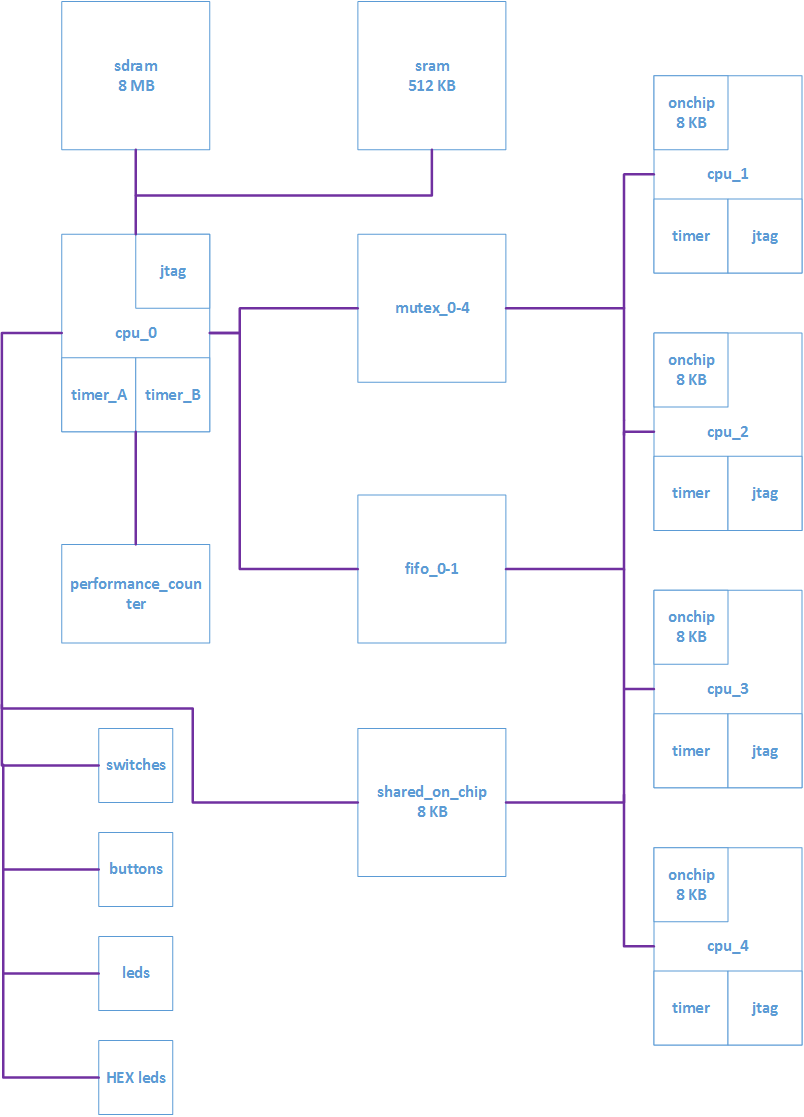
\includegraphics[scale=0.5]{interconnect.png}
	\label{fig1:SimplifiedInterconnectionGraph}
	\caption{Simplified interconnection graph.}
\end{figure}  
\subsection{CPUs}
There are five soft cores in the laboratory system, named from cpu\_0 to cpu\_4. Each core has its own timer(cpu\_0 owns two timers), jtag debug module and on-chip RAM.(Except cpu\_0 doesn't contain private on-chip memory) Additionally, cpu\_0 has its own performance counter to monitor execution time of code sections.
\subsection{Memory}
The system has \textbf{SDRAM, SRAM and on-chip memory}. The size of SDRAM is \textbf{8 MByte}, since the data address is 0x01000000 from to 0x017FFFFF. The size of SRAM is \textbf{512 KByte} and the address is 0x00080000 from to 0x000FFFFF. They are both exclusively connected to cpu\_0, which means they can only be accessed by cpu\_0. Each core except cpu\_0 has its own on-chip memory whose size is \textbf{8 KByte}. Additionally, there is a shared on-chip memory whose size is \textbf{8 KByte} that can be accessed by all the five cores.
\subsection{Peripherals}
\textbf{Eighteen} switches, \textbf{four} buttons, \textbf{eight} LED numeric displays, \textbf{nineteen} red LEDs and \textbf{eight} green LEDs are connected to cpu\_0. They can only be accessed by cpu\_0, which can be proved by the differentiation of \emph{system.h} files.
\subsection{Communication between cores}
There are three components to implement communication mechanisms: \textbf{shared on-chip memory, two FIFO memory cores, four mutexes}. These components are connected to the data interfaces of all the cores. Theses connections can be verified by the \emph{system.h} files.
%\subsection{Clock and reset}
%This part is not indicated in the simplified graph. All the components in the system are connect to the same clock and reset interface. Some components are also connected to jtag debug module reset interface for debugging.

\section{Communication Mechanisms}
As mentioned above, the system provides three hardware components---\textbf{shared on-chip memory, FIFO memory cores and mutexes} for inter-core communications.
\subsection{Read and write shared memory}
This mechanism is categorized by two method---\textbf{safe and unsafe  method}.
\subsubsection{Unsafe method} 
This is the simplest communication method between cores. There is a specific space in shared memory which can be accessed by address. Once one core writes data to the space and others can read the data through the address. This method comes with a huge potential risk. If the space is not ready to read(unwritten or uninitialized), it may cause fatal errors.
\begin{figure}[h]
	\centering
	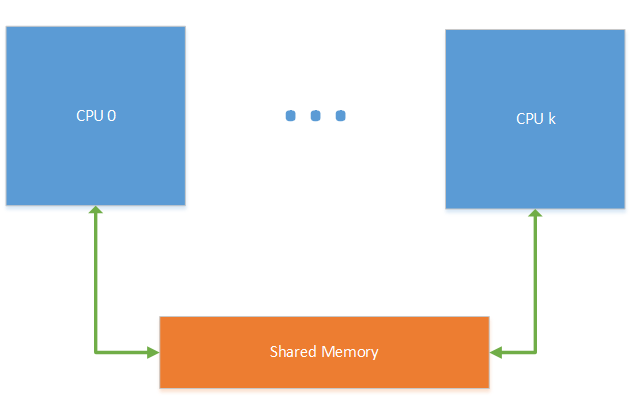
\includegraphics[scale=0.5]{sharedmemoryunsafe.png}
	\caption{Shared Memory in Unsafe Method}
	\label{fig:unsafe}
\end{figure}
\subsubsection{Safe method}
To avoid the reading issues, the safe method adds an extra 8-bit space as a  \textbf{flag}. When a data space is initialized or written, the corresponding flag is set to 1, which means "ready to be read". And after reading the data, the reader is responsible to set the flag to 0, which means "need to be written and can't be read". This method is a trade-off of space and security. 
\begin{figure}[h]
	\centering
	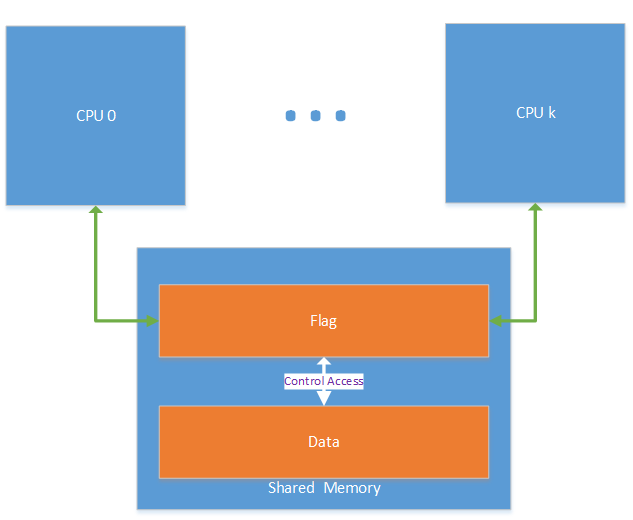
\includegraphics[scale=0.5]{sharedmemorysafe.png}
	\caption{Shared Memory in Safe Method}
	\label{fig:safe}
\end{figure}
\subsection{FIFO memory core}
FIFO, the abbreviation for \emph{"first in, first out"}, is a common data structure. The depth of FIFO memory cores in this system is 16, which means that the maximum 16 piece of 8-bit data can be buffered in every core. When the buffer is full,the cores can detect it and stop writing. Analogously, when the buffer is empty, the cores can also stop reading.
\begin{figure}[h]
	\centering
	\includegraphics[scale=0.5]{fifo.png}
	\caption{FIFO}
	\label{fig:fifo}
\end{figure}
\subsection{Mutex}
Mutex exclusion is a mechanism to avoid two or more threads or tasks running into the same critical section, such as accessing the same shared resource or responding to a timer\cite{courtois1971concurrent}. In our perception, the mutexes in this system are similar with semaphores. Not only in the aspect of function, but also locking mutex provides a blocking function. When a core or thread has locked a mutex, other cores or threads who try to lock the same mutex will be blocked until the mutex is finally unlocked. Additionally, we can also make locking a mutex non-blocking with a trylock function.
\begin{figure}[h]
	\centering
	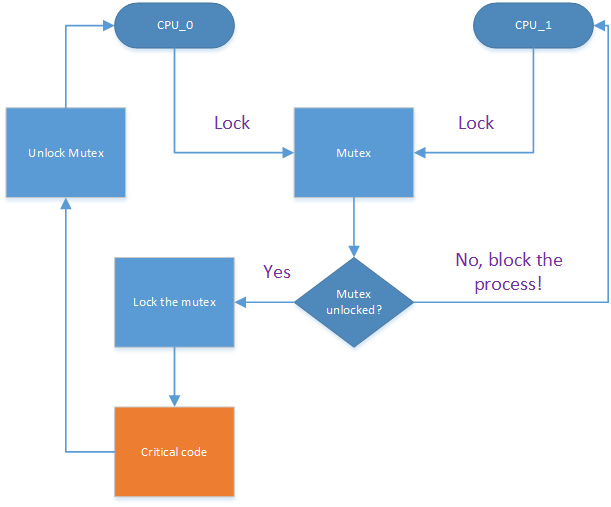
\includegraphics[scale=0.55]{mutex.png}
	\caption{Mutex}
	\label{fig:mutex}
\end{figure}
\section{Memory Footprint}
Memory footprint refers to the amount of main memory that a program uses or references while running. In the script of laboratory, \emph{nios2-elf-size} is included which is a command to show the code size of programs. The output of this command will contain five columns---\textbf{text, data, bss, dec, hex}.
\begin{itemize}
	\item{\textbf{text:}} the size of general code.
	\item{\textbf{data:}} the size of variables.
	\item{\textbf{bss:}} the size of uninitialized variables\cite{one1996smashing}.
	\item{\textbf{dec:}} the total size of the program, displayed in decimal.
	\item{\textbf{hex:}} the total size of the program, displayed in hexadecimal.
\end{itemize}
Finally, we put the result of our program in the terminal and the size unit of byte. According to the hardware description 
\begin{table}[h]
	\centering
	\caption{"Memory Footprint of Programs"}
	\label{tab:MemoryFootprint}
	\begin{tabular}{ccccccc}
		\toprule
		CPU& Memory& Text& Data &BSS& DEC& HEX\\
		\midrule
		cpu\_0& sram & 10448& 580& 424& 11452 & 2cbc\\
		cpu\_1& onchip& 1428& 96& 20& 1544& 608\\
		cpu\_2& onchip& 2704& 96& 20& 2820& b04\\
		cpu\_3& onchip& 2436& 96& 16& 2548& 9f4\\
		cpu\_4& onchip& 1312& 96& 16& 1424& 590\\
		\bottomrule
	\end{tabular}
\end{table}

\section{Demo Program}
As required, we designed a simple demo program to implement three inter-core mechanisms. In the following part, we will describe the five programs in the five cores.
\begin{figure*}
	\centering
	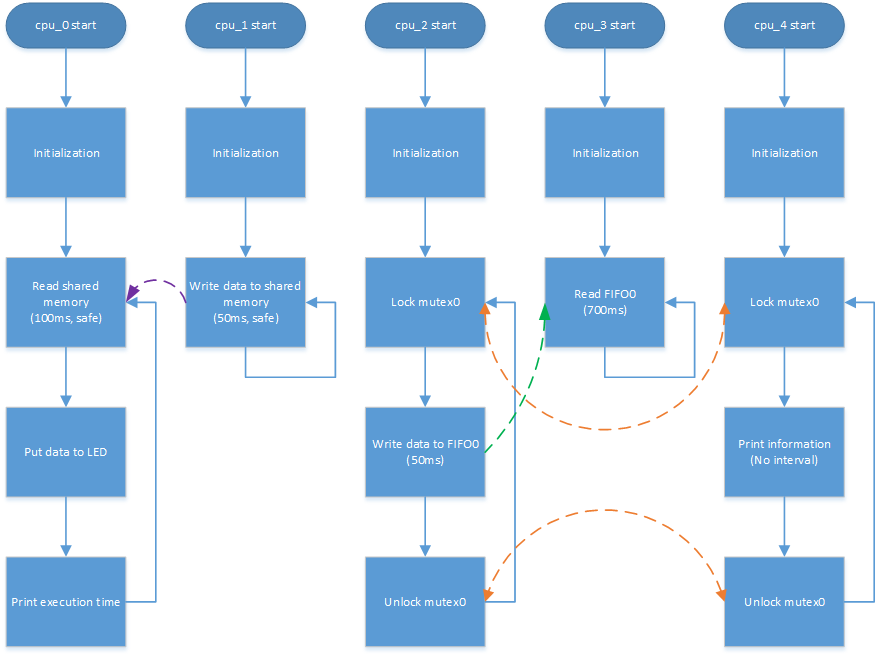
\includegraphics[scale=0.7]{program.png}
	\label{fig2:ProgramProcedureGraph}
	\caption{Program procedure graph for demo program}
\end{figure*}
\subsection{CPU 0}
Since cpu\_0 is connected with relatively more auxiliaries than other cores. We designed more function in cpu\_0.
\begin{itemize}
	\item{\textbf{Controlling LEDs, buttons and switches}}\\
	In every loop, the program will scan the statuses of buttons and switches. When a newly turned-on switch or a newly pressed-down button is detected, it will light the corresponding LED(s). Additionally, it will also store the status of switches in a variable for further use.
	\item{\textbf{Reading data from shared memory}}\\
	In this part, we implement safe method. First it uses FLAG to detect whether the shared memory is readable. If the program will read the data from VALUE and print it out. FLAG is at the start address of shared memory located in 0x00102000 and VALUE is located at the next address. If the part is unreadable, it will print a error message.
	\item{\textbf{Displaying information with LED numeric display}}\\
	There are two groups of LED numeric displays---HEX3\_HEX0 and HEX7\_HEX4. We use HEX3\_HEX0 to display the number indicated by switches and HEX7\_HEX4 for data read from shared memory.
	\item{\textbf{Monitoring execution time}}\\
	We use \emph{PERF\_BEGIN} and \emph{PERF\_END} to embrace the code section whose execution time we want to measure. And use \emph{perf\_print\_formatted\_report} to print out information we need.
\end{itemize}
\subsection{CPU 1}
The cpu\_1 writes to shared memory addressed at VALUE every 50ms if the content in FLAG is 0. This procure builds up the inter-core connection with cpu\_0.
\subsection{CPU 2}
After initialization, cpu\_2 will lock mutex\_0 and then write data to FIFO\_0 if it is not full every 50ms. And finally it will unlock mutex\_0.
\subsection{CPU 3}
Every 700ms, cpu\_3 will fetch data from FIFO\_0. If it is empty, it will give a error message.
\subsection{CPU 4}
At the beginning, cpu\_4 will try to lock mutex\_0. if it fails, it will be blocked. And after this, it will print a message without delay and unlock mutex\_0. The expected result is that the message is printed every 50ms due to the mutex-locking operations of cpu\_2.\\
\\
\indent
Since the time is limited, we only designed a simple demo program to demonstrate the three communication mechanisms. We will add more advanced functions in this program.\\
\indent
According to the lab manual, we drew a program procedure graph of this demo. In the figure, the purple arrow is for shared memory; the orange arrows are for mutexes; the green arrow is for FIFO.
\section{Optimizations for Space Usage}
Due to the limited resource in DE2 board, some optimizations are turned on to make the resulting program consume less space.
\subsection{Os optimization level}
Os level is enabled to optimize space usage (code and data) of resulting program. -Os enables all -O2 optimizations that do not typically increase code size. It also performs further optimizations designed to reduce code size\cite{osGNUlevel}.
\subsection{Small C library}
Small C library is also enabled with . This reduces code and data footprint at the expense of reduced functionality. Several newlib features are removed such as floating-point support in printf(), stdin input routines, and buffered I/O.
\subsection{Reduced device drivers}
Certain drivers are compiled with reduced functionality to reduce code footprint.
\subsection{Lightweight device driver API}
Lightweight device driver API is enabled. This reduces code and data footprint by removing the HAL layer that maps device names (e.g. /dev/uart0) to file descriptors. Instead, driver routines are called directly.
\subsection{C++ support}
C++ support is disabled to reduce code footprint.
\subsection{Clean exit}
Code footprint can be reduced by disabling clean exit.
\section{Summary}
Through this laboratory, we reviewed the NIOS II labs in Embedded Systems course and got a basic of multiprocessor system development. Finishing this lab is a good beginning of the following labs.

% An example of a floating figure using the graphicx package.
% Note that \label must occur AFTER (or within) \caption.
% For figures, \caption should occur after the \includegraphics.
% Note that IEEEtran v1.7 and later has special internal code that
% is designed to preserve the operation of \label within \caption
% even when the captionsoff option is in effect. However, because
% of issues like this, it may be the safest practice to put all your
% \label just after \caption rather than within \caption{}.
%
% Reminder: the "draftcls" or "draftclsnofoot", not "draft", class
% option should be used if it is desired that the figures are to be
% displayed while in draft mode.
%
%\begin{figure}[!t]
%\centering
%\includegraphics[width=2.5in]{myfigure}
% where an .eps filename suffix will be assumed under latex, 
% and a .pdf suffix will be assumed for pdflatex; or what has been declared
% via \DeclareGraphicsExtensions.
%\caption{Simulation results for the network.}
%\label{fig_sim}
%\end{figure}

% Note that the IEEE typically puts floats only at the top, even when this
% results in a large percentage of a column being occupied by floats.


% An example of a double column floating figure using two subfigures.
% (The subfig.sty package must be loaded for this to work.)
% The subfigure \label commands are set within each subfloat command,
% and the \label for the overall figure must come after \caption.
% \hfil is used as a separator to get equal spacing.
% Watch out that the combined width of all the subfigures on a 
% line do not exceed the text width or a line break will occur.
%
%\begin{figure*}[!t]
%\centering
%\subfloat[Case I]{\includegraphics[width=2.5in]{box}%
%\label{fig_first_case}}
%\hfil
%\subfloat[Case II]{\includegraphics[width=2.5in]{box}%
%\label{fig_second_case}}
%\caption{Simulation results for the network.}
%\label{fig_sim}
%\end{figure*}
%
% Note that often IEEE papers with subfigures do not employ subfigure
% captions (using the optional argument to \subfloat[]), but instead will
% reference/describe all of them (a), (b), etc., within the main caption.
% Be aware that for subfig.sty to generate the (a), (b), etc., subfigure
% labels, the optional argument to \subfloat must be present. If a
% subcaption is not desired, just leave its contents blank,
% e.g., \subfloat[].


% An example of a floating table. Note that, for IEEE style tables, the
% \caption command should come BEFORE the table and, given that table
% captions serve much like titles, are usually capitalized except for words
% such as a, an, and, as, at, but, by, for, in, nor, of, on, or, the, to
% and up, which are usually not capitalized unless they are the first or
% last word of the caption. Table text will default to \footnotesize as
% the IEEE normally uses this smaller font for tables.
% The \label must come after \caption as always.
%
%\begin{table}[!t]
%% increase table row spacing, adjust to taste
%\renewcommand{\arraystretch}{1.3}
% if using array.sty, it might be a good idea to tweak the value of
% \extrarowheight as needed to properly center the text within the cells
%\caption{An Example of a Table}
%\label{table_example}
%\centering
%% Some packages, such as MDW tools, offer better commands for making tables
%% than the plain LaTeX2e tabular which is used here.
%\begin{tabular}{|c||c|}
%\hline
%One & Two\\
%\hline
%Three & Four\\
%\hline
%\end{tabular}
%\end{table}


% Note that the IEEE does not put floats in the very first column
% - or typically anywhere on the first page for that matter. Also,
% in-text middle ("here") positioning is typically not used, but it
% is allowed and encouraged for Computer Society conferences (but
% not Computer Society journals). Most IEEE journals/conferences use
% top floats exclusively. 
% Note that, LaTeX2e, unlike IEEE journals/conferences, places
% footnotes above bottom floats. This can be corrected via the
% \fnbelowfloat command of the stfloats package.


%\newpage
%\begin{figure*}
%	\centering
%	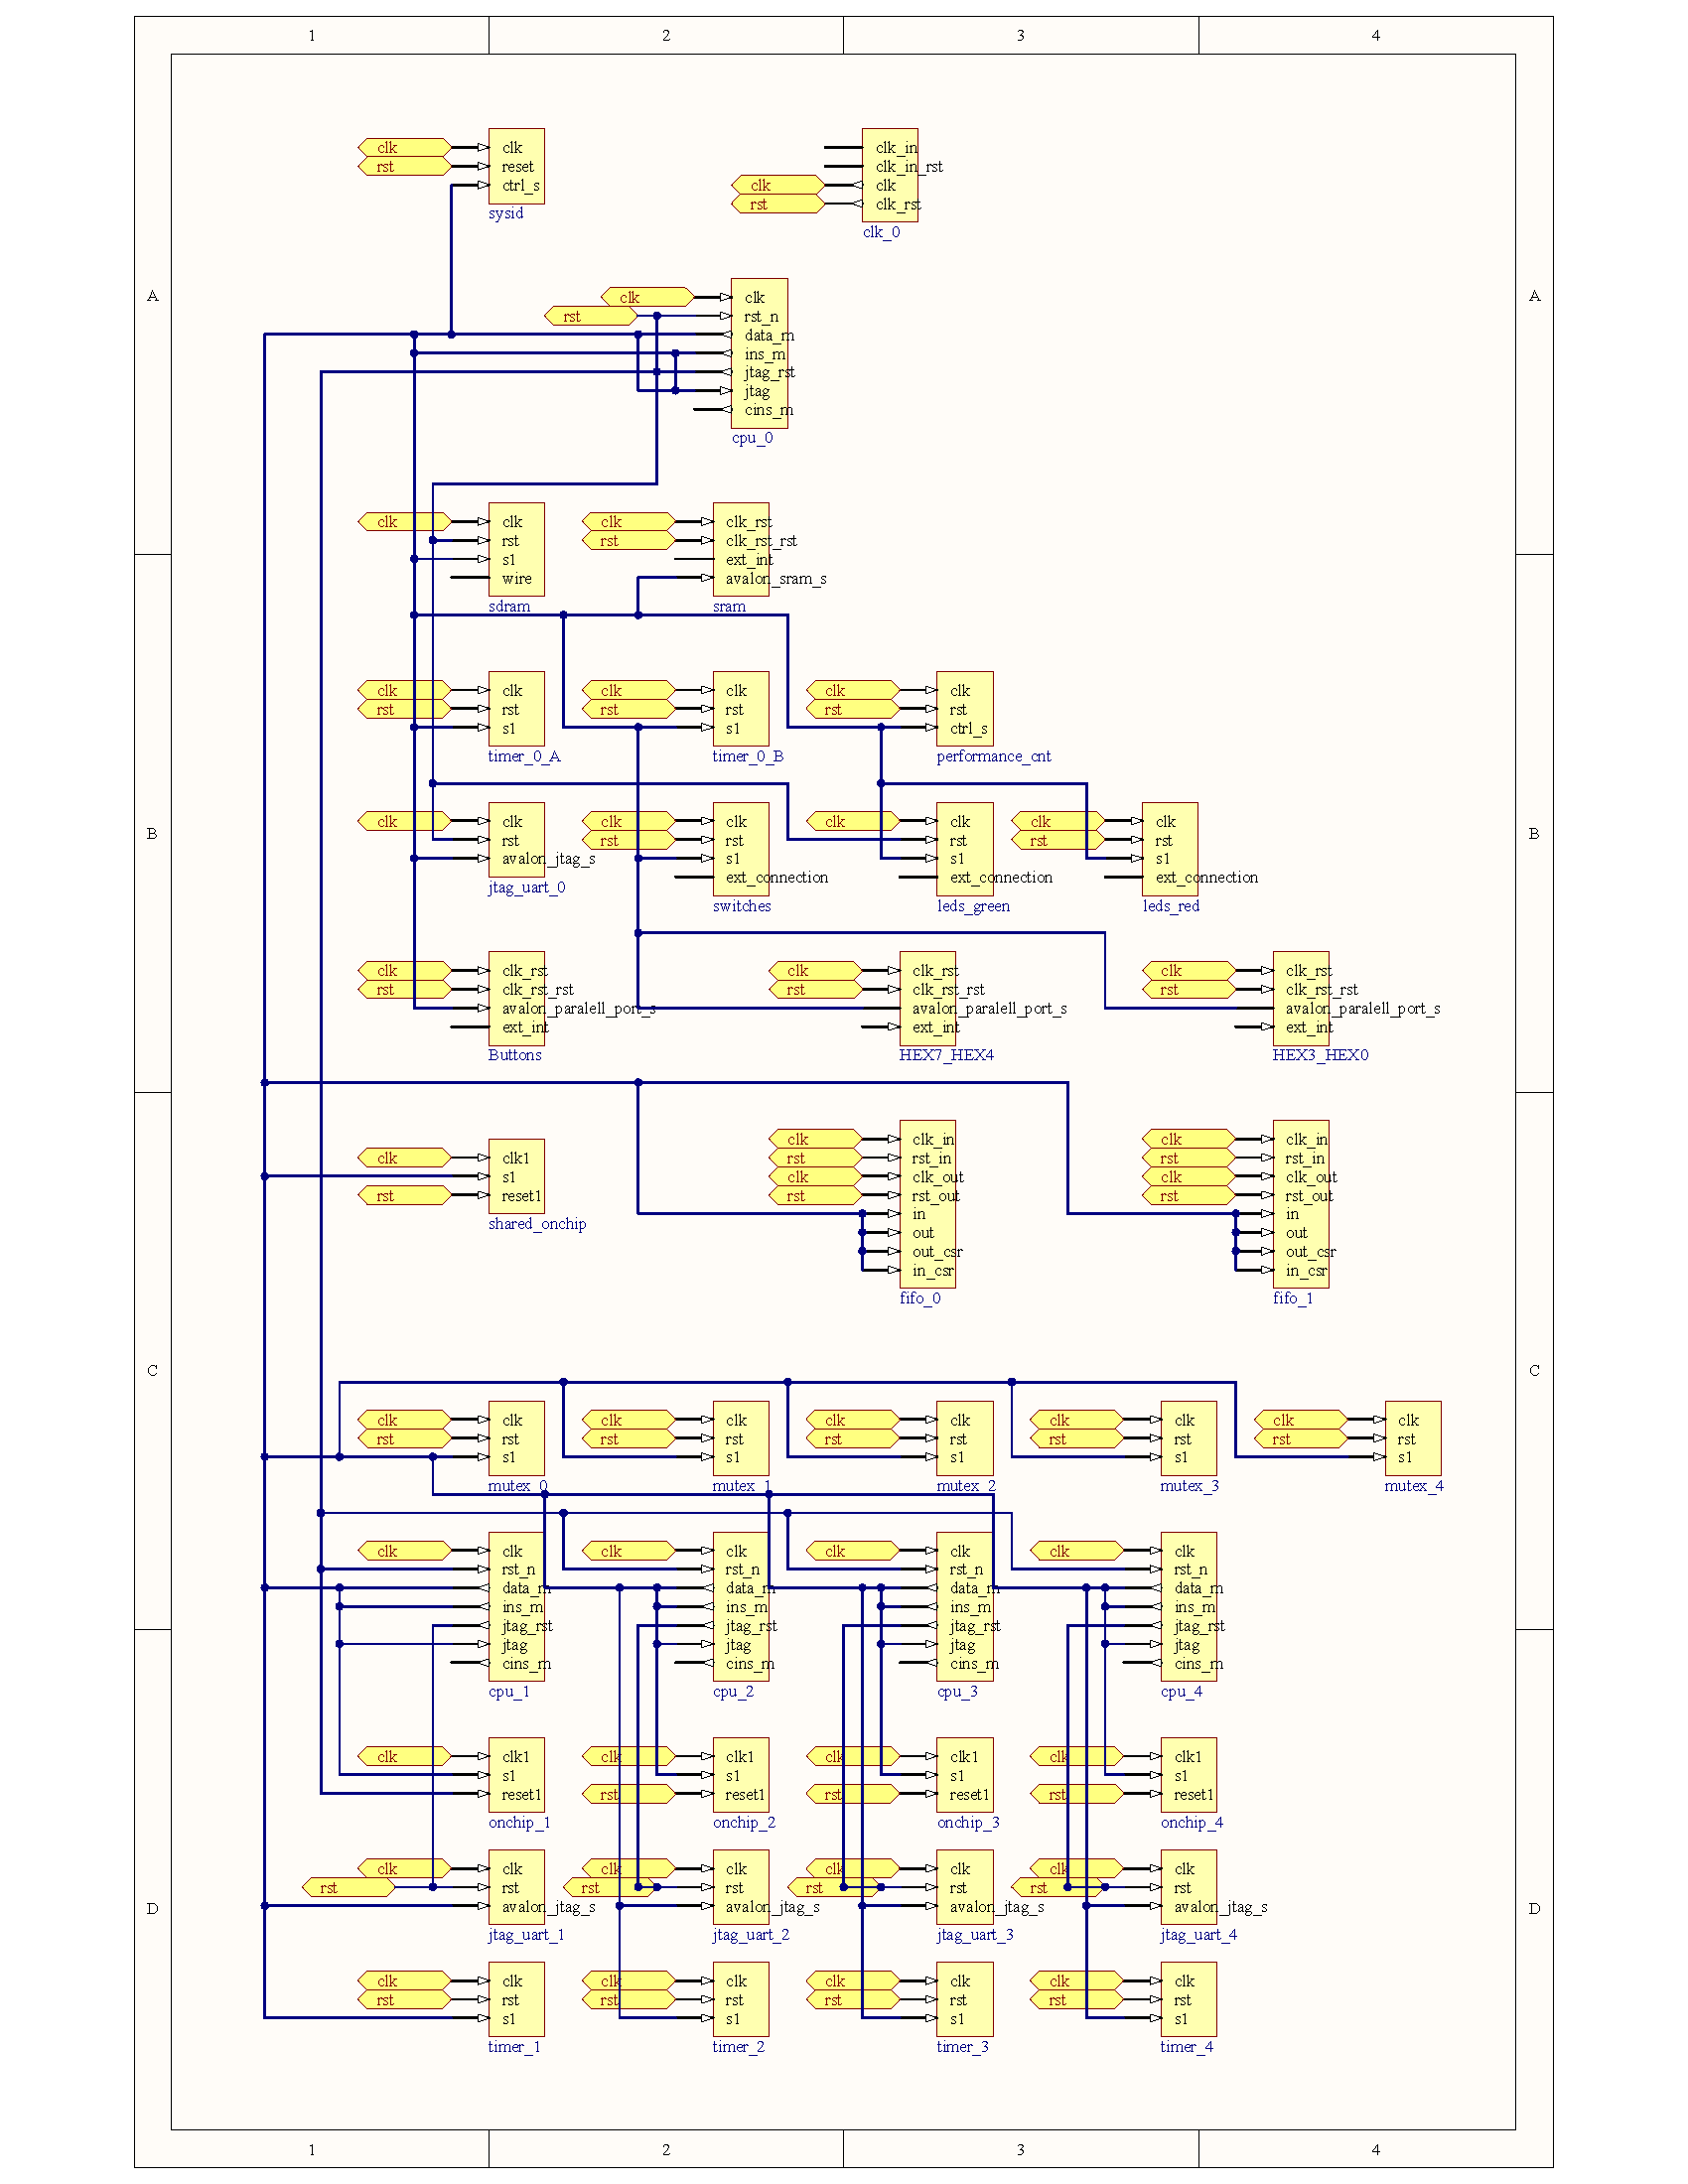
\includegraphics[scale=0.87]{SchematicPrints.png}
%	\caption{Detailed Interconnection Graph}
%	\label{SchematicPrints}
%\end{figure*}





% trigger a \newpage just before the given reference
% number - used to balance the columns on the last page
% adjust value as needed - may need to be readjusted if
% the document is modified later
%\IEEEtriggeratref{8}
% The "triggered" command can be changed if desired:
%\IEEEtriggercmd{\enlargethispage{-5in}}

% references section

% can use a bibliography generated by BibTeX as a .bbl file
% BibTeX documentation can be easily obtained at:
% http://mirror.ctan.org/biblio/bibtex/contrib/doc/
% The IEEEtran BibTeX style support page is at:
% http://www.michaelshell.org/tex/ieeetran/bibtex/
\bibliographystyle{IEEEtran}
% argument is your BibTeX string definitions and bibliography database(s)
\bibliography{bibi}
%
% <OR> manually copy in the resultant .bbl file
% set second argument of \begin to the number of references
% (used to reserve space for the reference number labels box)
%\newpage
%\appendix
%\begin{figure*}
%	\centering
%	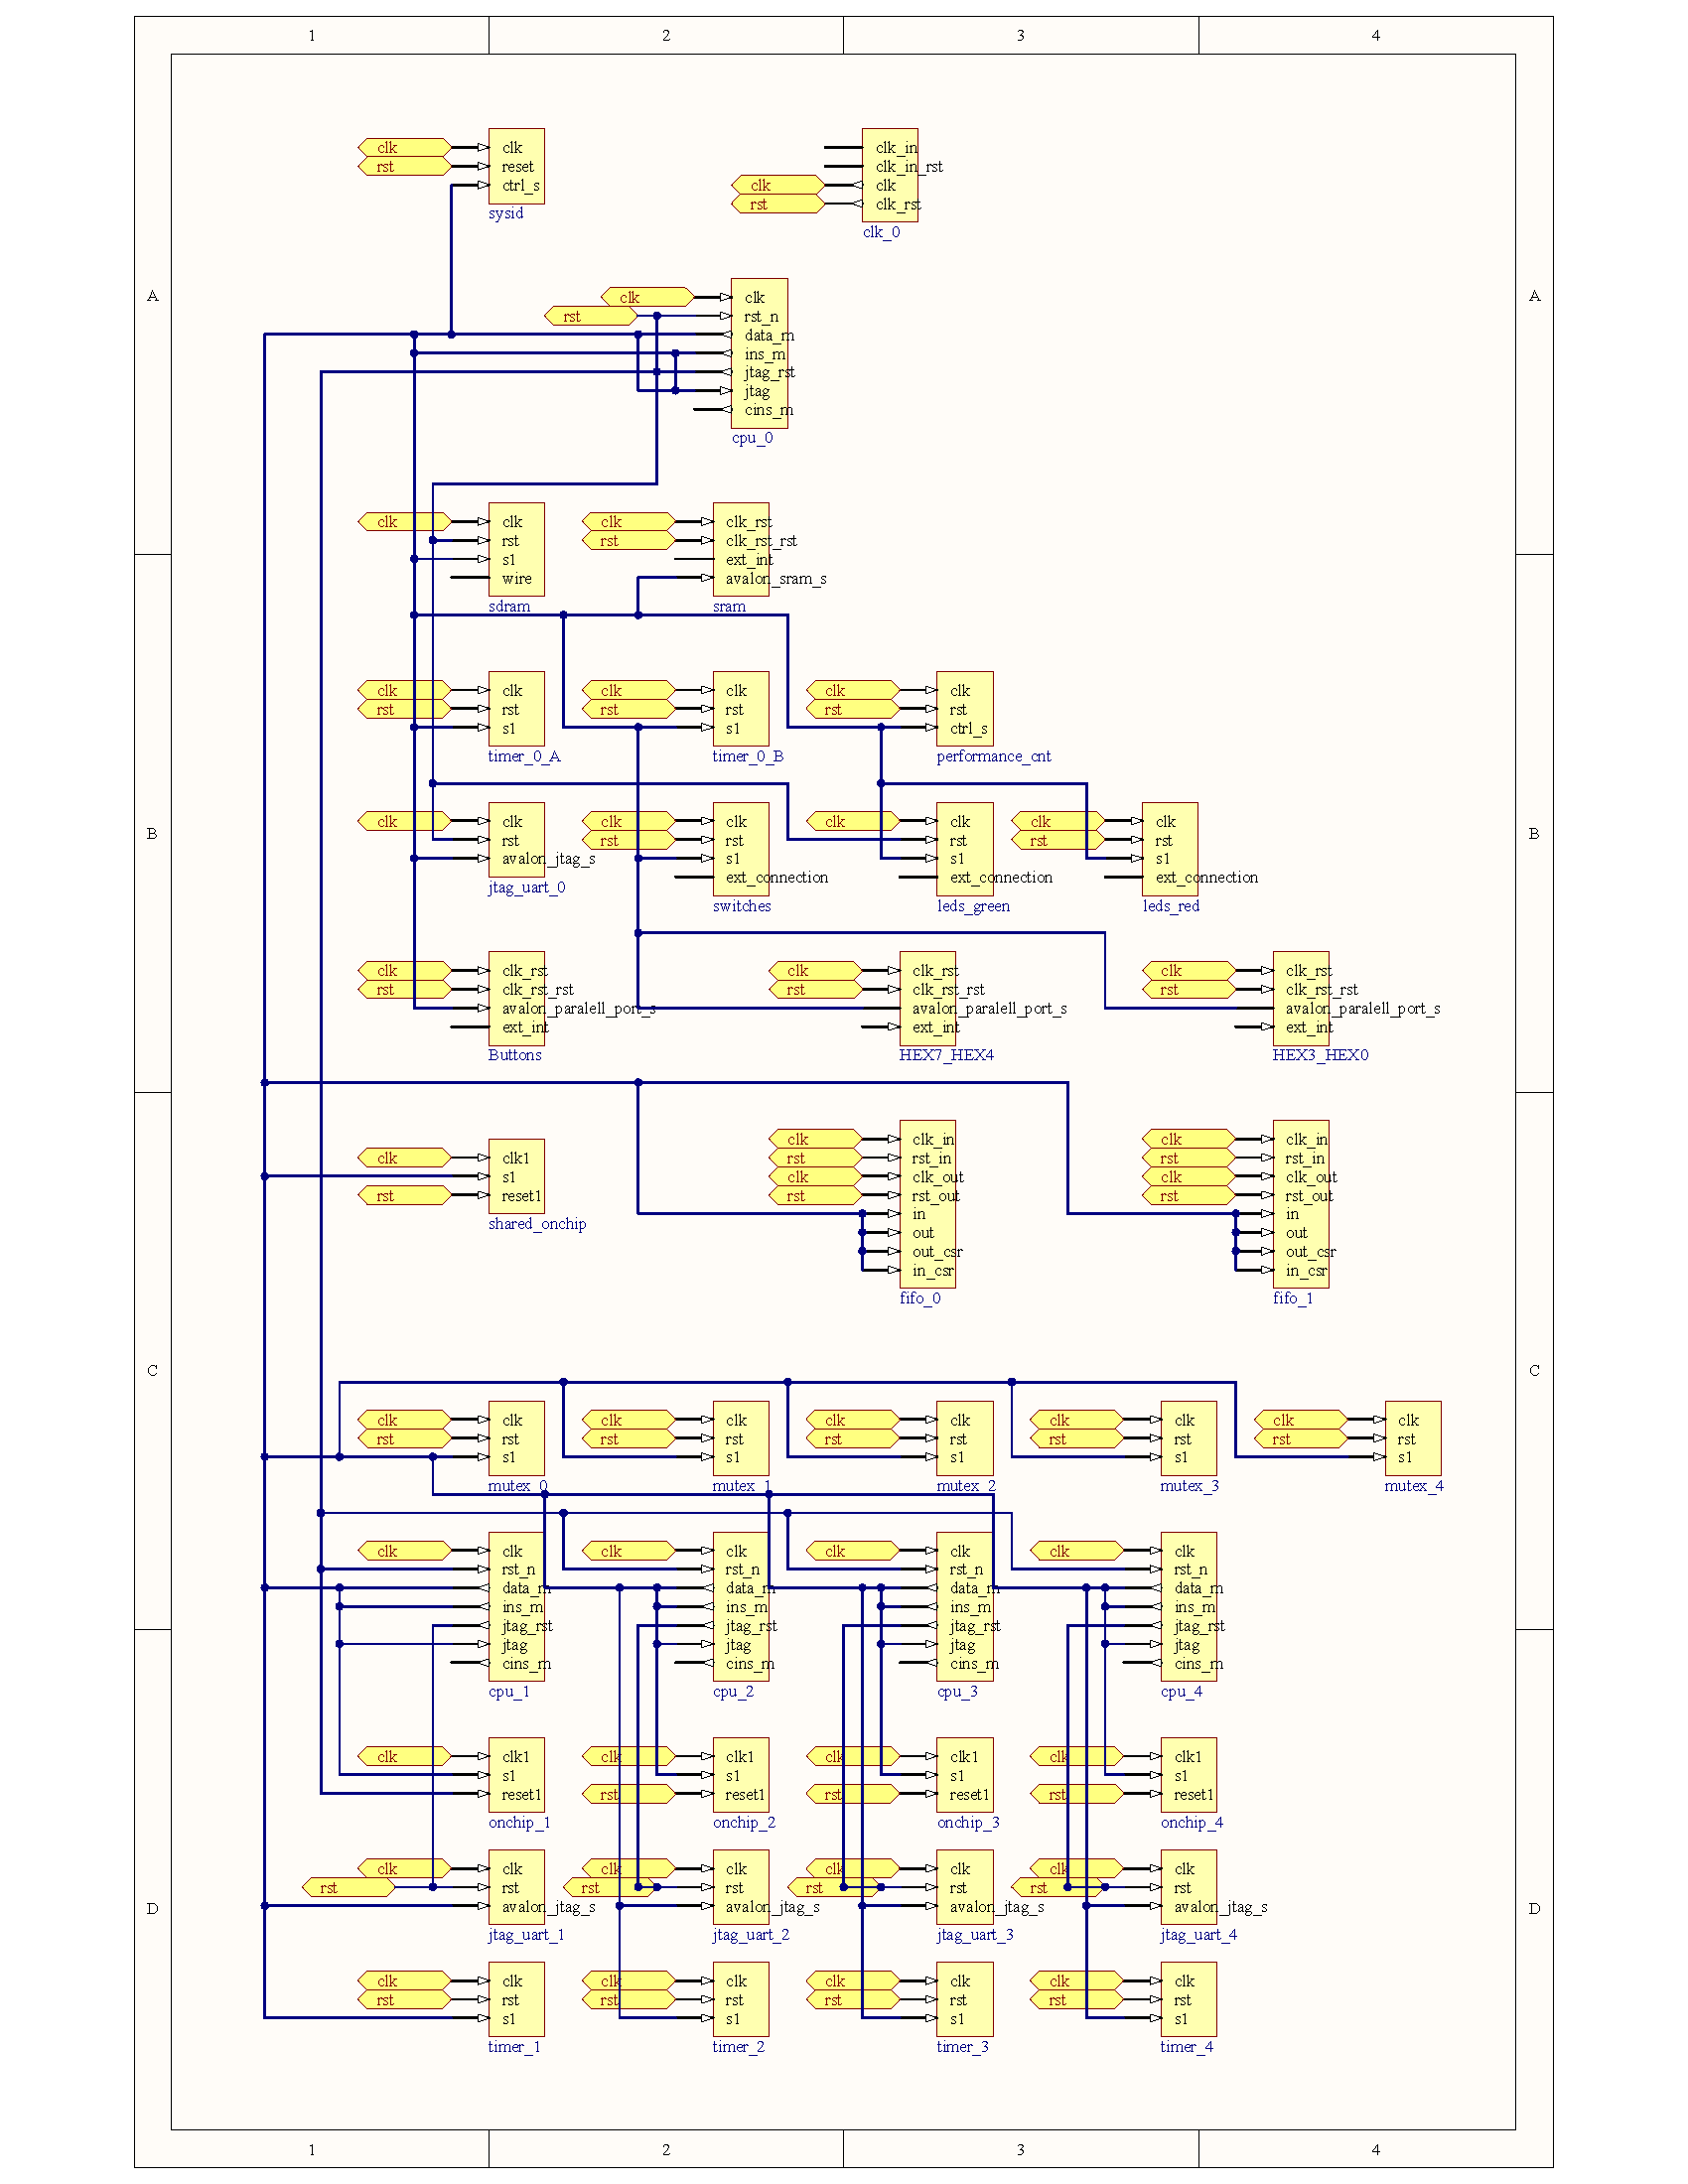
\includegraphics[scale=0.87]{SchematicPrints.png}
%	\caption{Detailed Interconnection Graph}
%	\label{SchematicPrints}
%\end{figure*}





% that's all folks
\end{document}



%%% Local Variables:
%%% mode: latex
%%% TeX-master: t
%%% End:
